\documentclass{CPSPresentation}
%\documentclass[uselowcontrast]{CPSPresentation}

\usepackage[portuguese]{babel}
\usepackage[T1]{fontenc} % Output font encoding for international characters
\usepackage[utf8]{inputenc} % Required for inputting international characters

\usepackage{XCharter} % Use the XCharter font
\AtBeginDocument{\fontsize{12}{12}\selectfont}
\newcommand{\link}[2]{{\color{MULTurquoise}\href{#1}{\textit{#2}}}}

\geometry{papersize={210mm,150mm}}
\usepackage{caption}
\usepackage{siunitx}
\usepackage{pdfpages}
\usepackage{booktabs}
\usepackage{multirow}
\usefonttheme[]{serif}
\usepackage{amsmath, latexsym, color, graphicx, amssymb, bm, here}
\usepackage{epsf, epsfig, pifont,tikz,subfigure}
\usepackage{graphics, calrsfs}
\usepackage{times}
\usepackage{fancybox,calc}
\usepackage{palatino,mathpazo}
\usepackage{amsfonts}
\usepackage{wrapfig}
\usepackage{multicol}
\usepackage{sidecap}
\usepackage{academicons}
%\usepackage{pdfauthor}
%\usepackage{pdfcreator}
\usepackage{hyperref}
\usepackage{listings}
\usepackage[portuguese]{babel}
\usepackage[]{hyperref}
\usepackage{float}
\usepackage{amsmath}
\usepackage{setspace}


\title[Minicurso FPGAs]{\huge Introdução ao Quartus II} 


\author[Prof. Dr. Oscar Eduardo Anacona Mosquera]{Prof. Dr. Oscar Eduardo Anacona Mosquera \newline\newline 
\scriptsize{oscar.mosquera@ufmt.br}
}

\AtBeginSection[]
{
	\begin{frame}{Conteúdo}
		\tableofcontents[currentsection]
	\end{frame}
}


\begin{document}

\begin{frame}[plain]
\titlepage
%\vspace{3cm}
%\begin{center} \color{MULTurquoise} {Chair of Cyber-Physical-Systems}\end{center}

\end{frame}




\section{Objetivos}

%%====================================================================================
\begin{frame}
	\frametitle{Objetivos}
	
	\begin{itemize}
		\item \textbf{Introdução ao Software Quartus:}
		\begin{itemize}
			\item Familiarizar os participantes com o ambiente de desenvolvimento Quartus da Intel (anteriormente Altera).
			\item Explorar as principais características e funcionalidades do software para design de circuitos digitais em FPGA.
		\end{itemize}
		
		\item \textbf{Metodologia de Projeto em Quartus:}
		\begin{itemize}
			\item Apresentar uma metodologia de projeto passo a passo para desenvolver projetos em Quartus.
		\end{itemize}
		
		\item \textbf{Tutorial de Criação de Projetos em Quartus:}
		\begin{itemize}
			\item Guiar os participantes através de um tutorial prático para criar um projeto simples em Quartus.
			\item Demonstrar como criar e configurar um projeto, adicionar arquivos de design, compilar e sintetizar o código, e programar um dispositivo FPGA.
		\end{itemize}
	\end{itemize}
\end{frame}
%%====================================================================================

\section{Introdução aos dispositivos e software de design da Altera}

%%====================================================================================
\begin{frame}{Software Quartus II}
	
\begin{block}{}
	\justifying
	O Quartus é uma suíte de software desenvolvida pela Altera Corporation, que agora faz parte da Intel FPGA. Essa ferramenta é amplamente utilizada no projeto e programação de dispositivos lógicos programáveis como FPGAs (\textbf{Field-Programmable Gate Arrays}).
	
\end{block}	
	
	
	\begin{figure}[h]
		\centering
		\includegraphics[width=0.97\textwidth]{Figs/fig02.png}
	\end{figure}
	
\end{frame}
%%====================================================================================
%%====================================================================================
\begin{frame}
	\frametitle{Software Quartus II}

	
	Aqui estão alguns dos principais componentes e recursos do Quartus:
	
	\begin{itemize}
		\justifying
		\setbeamertemplate{itemize item}[triangle]
		\item \textbf{Ambiente de Desenvolvimento Integrado (IDE):} O Quartus fornece um ambiente integrado para design, compilação, simulação e programação de dispositivos FPGA. Ele possui uma interface gráfica de usuário (GUI) que permite aos projetistas criar e modificar seus projetos de forma eficiente.
		
		\item \textbf{Editor de Design Gráfico:} O Quartus inclui um editor gráfico que permite aos usuários criar esquemáticos para seus projetos. Esse editor suporta a criação de designs digitais utilizando elementos lógicos, como portas lógicas, flip-flops e outros blocos.
		
		\item \textbf{Compilador Quartus:} O compilador do Quartus converte o design do usuário em um formato que pode ser implementado no FPGA. Ele otimiza o design, faz a alocação de recursos no FPGA e gera os arquivos de configuração necessários para a programação do dispositivo.
		
		\item \textbf{Simulador de Hardware:} O Quartus inclui um simulador que permite aos projetistas verificar o comportamento do seu design antes de implementá-lo no hardware real. Isso ajuda a identificar possíveis problemas e aperfeiçoar o design antes da etapa de implementação.
		
		\item \textbf{Analisador de Timing:} Este recurso permite a análise do timing do design, garantindo que todas as restrições de temporização sejam atendidas para garantir o funcionamento adequado do circuito.
	\end{itemize}
	
	
\end{frame}
%%====================================================================================

%%====================================================================================
\begin{frame}{Software Quartus II}
	\justifying
	
	\begin{block}{}
	\justifying
	Ferramenta de desenvolvimento totalmente integrada.
	
	
		\begin{itemize}
		\item Múltiplos métodos de entrada de design
		\item Síntese lógica
		\item Place and route
		\item Static timing analysis
		\item Análise de potência e SSN (Simultaneous Switching Noise)
		\item Programação de dispositivos
		\end{itemize}
	\end{block}
	
	\begin{alertblock}{}
	Oferece suporte a ferramentas de simulação HDL padrão.
	\begin{itemize}
	\item Inclui a ferramenta ModelSim-Altera Starter Edition
	\item Atualização opcional para a ferramenta ModelSim-Altera Edition
	\end{itemize}

	\end{alertblock}	
	
	
\end{frame}
%%====================================================================================
%%====================================================================================
\begin{frame}{Software Quartus II}
	\justifying
	
	\begin{block}{}
	\justifying	
	\begin{itemize}
		\item MegaWizard Plug-In Manager and Qsys design tools
		\item TimeQuest Timing Analyzer
		\item PowerPlay Power Analyzer
		\item Static timing analysis
		\item 32 and 64-bit Windows and Linux support
		\item Multi-processor support
		\item Licenças fixas e flutuantes
	\end{itemize}
	\end{block}

	
	\begin{alertblock}{}
	Disponível em \href{https://www.intel.com/content/www/us/en/software-kit/666221/intel-quartus-ii-web-edition-design-software-version-13-1-for-windows.html/}{\beamergotobutton{Link}}
	\end{alertblock}	
	
	
\end{frame}
%%====================================================================================
\section{Metodologia}
%%====================================================================================
\begin{frame}{Metodologia}
	\justifying
	
	\begin{figure}[h]
		\centering
		\includegraphics[width=0.97\textwidth]{Figs/fig08.png}
	\end{figure}
	
	
\end{frame}
%%====================================================================================
%%====================================================================================
\begin{frame}{Metodologia}
	\justifying
	
	\begin{figure}[h]
		\centering
		\includegraphics[width=0.97\textwidth]{Figs/fig09.png}
	\end{figure}
	
	
\end{frame}
%===================================================================================================
\section{Quartus II interface}
%===================================================================================================
\begin{frame}
	\frametitle{Quartus II interface}
	
	\begin{block}{}
		\justifying
		Quartus II Software
	\end{block}
	
	
	
	\begin{figure}[h]
		\centering
		\includegraphics[width=1.01\textwidth]{quartus/fig02.pdf}
	\end{figure}
	
	
\end{frame}
%===================================================================================================

%%====================================================================================
\begin{frame}
	\frametitle{Quartus II interface}
	
	
	\begin{block}{}
		\justifying
		Quartus II Software
	\end{block}
	
	
	
	
	\begin{figure}[h]
		\centering
		\includegraphics[width=1.02\textwidth]{quartus/fig03.pdf}
	\end{figure}
	
	
\end{frame}
%===================================================================================================

%%====================================================================================
\begin{frame}
	\frametitle{Quartus II interface}
	
	\begin{block}{}
		\justifying
		Ambiente operacional padrão do Quartus II
	\end{block}
	
	\begin{figure}[h]
		\centering
		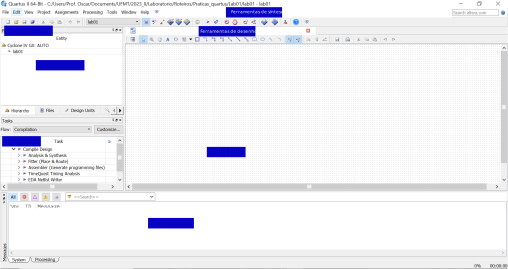
\includegraphics[width=1.02\textwidth]{quartus/fig04.pdf}
	\end{figure}
	
	
\end{frame}
%%====================================================================================
%%====================================================================================
\begin{frame}{Quartus II interface}
	\justifying
	
	\begin{figure}[h]
			\centering
			\includegraphics[width=0.97\textwidth]{Figs/fig05.png}
		\end{figure}
	
	
\end{frame}
%%====================================================================================
%%====================================================================================
\begin{frame}{Quartus II interface}
	\justifying
	
	\begin{figure}[h]
			\centering
			\includegraphics[width=0.97\textwidth]{Figs/fig06.png}
		\end{figure}
	
	
\end{frame}
%%====================================================================================
\subsection{Criação de projeto}
%====================================================================================
\begin{frame}
	\frametitle{Criação de um novo projeto}
	
	\begin{block}{}
		\justifying
		Criar um novo projeto para o desenho de um circuito digital
	\end{block}
	
	\begin{figure}[h]
		\centering
		\includegraphics[width=1.02\textwidth]{quartus/fig07.png}
	\end{figure}
	
	
\end{frame}
%%====================================================================================
%%====================================================================================
\begin{frame}
	\frametitle{Criação de um novo projeto}
	
	\begin{block}{}
		\justifying
		Criar um novo projeto para o desenho de um circuito digital
	\end{block}
	
	\begin{figure}[h]
		\centering
		\includegraphics[width=1.02\textwidth]{quartus/fig08.png}
	\end{figure}
	
	
\end{frame}
%%====================================================================================
%%====================================================================================
\begin{frame}
	\frametitle{Criação de um novo projeto}
	
	\begin{block}{}
		\justifying
		Escolher uma pasta para guardar seu projeto, não use acentos, nem espaço, e nem caracteres especiais para nomear o projeto
	\end{block}
	
	\begin{figure}[h]
		\centering
		\includegraphics[width=1.02\textwidth]{quartus/fig09.png}
	\end{figure}
	
	
\end{frame}
%%====================================================================================
%%====================================================================================
\begin{frame}
	\frametitle{Criação de um novo projeto}
	
	
	\begin{figure}[h]
		\centering
		\includegraphics[width=1.02\textwidth]{quartus/fig10.png}
	\end{figure}
	
	
\end{frame}

%%====================================================================================
%%====================================================================================
\begin{frame}
	\frametitle{Criação de um novo projeto}
	
	\begin{block}{}
		\justifying
		Escolher qualquer plataforma
	\end{block}
	
	\begin{figure}[h]
		\centering
		\includegraphics[width=1.02\textwidth]{quartus/fig23.pdf}
	\end{figure}
	
	
\end{frame}
%%====================================================================================
%%====================================================================================
\begin{frame}
	\frametitle{Criação de um novo projeto}
	
	\begin{block}{}
		\justifying
		Escolher a ferramenta de simulação
	\end{block}
	
	\begin{figure}[h]
		\centering
		\includegraphics[width=1.02\textwidth]{quartus/fig24.pdf}
	\end{figure}
	
	
\end{frame}
%%====================================================================================
%%====================================================================================
\begin{frame}
	\frametitle{Criação de um novo projeto}
	
	\begin{block}{}
		\justifying
		Resumo das configurações do projeto
	\end{block}
	
	\begin{figure}[h]
		\centering
		\includegraphics[width=1.02\textwidth]{quartus/fig25.pdf}
	\end{figure}
	
	
\end{frame}

%===================================================================================================
\subsection{Criação do esquemáticos}
%===================================================================================================

\begin{frame}
	\frametitle{Configuração da ferramenta de simulação}
	
	\begin{block}{}
		\justifying
		Caso você não tenha configurado a ferramenta de simulação durante a criação do projeto
	\end{block}
	
	\begin{figure}[h]
		\centering
		\includegraphics[width=1.02\textwidth]{quartus/fig22.pdf}
	\end{figure}
	
	
\end{frame}
%%====================================================================================
%%====================================================================================
\begin{frame}
	\frametitle{Ferramentas de desenho de esquemáticos}
	
	\begin{block}{}
		\justifying
		Criar um novo esquemático para desenhar o circuito lógico
	\end{block}
	
	\begin{figure}[h]
		\centering
		\includegraphics[width=1.02\textwidth]{quartus/fig26.pdf}
	\end{figure}
	
	
\end{frame}
%%====================================================================================
%%====================================================================================
\begin{frame}
	\frametitle{Área de trabalho do Quartus}
	
	\begin{block}{}
		\justifying
		Ambiente de desenvolvimento
	\end{block}
	
	\begin{figure}[h]
		\centering
		\includegraphics[width=1.02\textwidth]{quartus/fig16.png}
	\end{figure}
	
	
\end{frame}
%%====================================================================================
%%====================================================================================
\begin{frame}
	\frametitle{Área de trabalho do Quartus}
	
	\begin{block}{}
		\justifying
		Ambiente de desenvolvimento
	\end{block}
	
	\begin{figure}[h]
		\centering
		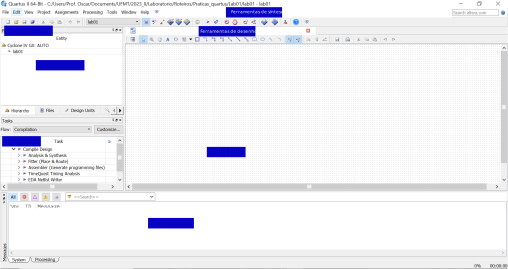
\includegraphics[width=1.02\textwidth]{quartus/fig04.pdf}
	\end{figure}
	
	
\end{frame}
%%====================================================================================
%%====================================================================================

\begin{frame}
	\frametitle{Ferramentas de desenho de esquemáticos}
	
	\begin{block}{}
		\justifying
		Podem-se usar esses ícones para implementar os circuitos lógicos
	\end{block}
	
	\begin{figure}[h]
		\centering
		\includegraphics[width=0.58\textwidth]{quartus/fig17.png}
	\end{figure}
	
	\begin{enumerate}
		\item Vincula/desvincula a janela de desenho do modulo principal
		\item Ponteiro do cursor do mouse
		\item Lupa para zoom in e zoom out
		\item Caixa de edição para textos na área de desenho
		\item \textbf{Botão para abrir a biblioteca de componentes}
		\item \textbf{Pin tool} é para criar os sinais de entrada/intermediarias/saída
		\item Fio simples para conexão entre componentes
		\item Barramento simples para conexões entre componentes
		\item Barramento múltiplo para conexões entre componentes
		\item Ferramentas de rotação de componentes da área de desenho
		\item Ferramentas de desenhos simples
		
		
	\end{enumerate}
	
\end{frame}
%%====================================================================================
%%====================================================================================
\begin{frame}
	\frametitle{Desenho de um circuito lógico}
	
	\begin{block}{}
		\justifying
		Ambiente de desenvolvimento
	\end{block}
	
	\begin{figure}[h]
		\centering
		\includegraphics[width=1.02\textwidth]{quartus/fig05.pdf}
	\end{figure}
	
	
\end{frame}

%%====================================================================================

%%====================================================================================
\begin{frame}
	\frametitle{Desenho de um circuito lógico}
	
	
	\begin{figure}[h]
		\centering
		\includegraphics[width=1.02\textwidth]{quartus/fig06.pdf}
	\end{figure}
	
	
\end{frame}
%%====================================================================================
%%====================================================================================
\begin{frame}
	\frametitle{Desenho de um circuito lógico}
	
	
	\begin{figure}[h]
		\centering
		\includegraphics[width=1.02\textwidth]{quartus/fig07.pdf}
	\end{figure}
	
	
\end{frame}
%%====================================================================================
%%====================================================================================
\begin{frame}
	\frametitle{Desenho de um circuito lógico}
	
	
	\begin{figure}[h]
		\centering
		\includegraphics[width=1.02\textwidth]{quartus/fig08.pdf}
	\end{figure}
	
	
\end{frame}
%%====================================================================================
%%====================================================================================
\begin{frame}
	\frametitle{Desenho de um circuito lógico}
	
	
	\begin{figure}[h]
		\centering
		\includegraphics[width=1.02\textwidth]{quartus/fig09.pdf}
	\end{figure}
	
	
\end{frame}
%%====================================================================================
%%====================================================================================
\begin{frame}
	\frametitle{Desenho de um circuito lógico}
	
	
	\begin{figure}[h]
		\centering
		\includegraphics[width=1.02\textwidth]{quartus/fig10.pdf}
	\end{figure}
	
	
\end{frame}
%%====================================================================================
%%====================================================================================
\begin{frame}
	\frametitle{Desenho de um circuito lógico}
	
	
	\begin{figure}[h]
		\centering
		\includegraphics[width=1.02\textwidth]{quartus/fig11.pdf}
	\end{figure}
	
	
\end{frame}
%%====================================================================================
%%====================================================================================
\begin{frame}
	\frametitle{Desenho de um circuito lógico}
	
	
	\begin{figure}[h]
		\centering
		\includegraphics[width=1.02\textwidth]{quartus/fig12.pdf}
	\end{figure}
	
	
\end{frame}
%%====================================================================================
%%====================================================================================
\begin{frame}
	\frametitle{Desenho de um circuito lógico}
	
	
	\begin{figure}[h]
		\centering
		\includegraphics[width=1.02\textwidth]{quartus/fig13.pdf}
	\end{figure}
	
	
\end{frame}
%%====================================================================================
%%====================================================================================

\begin{frame}
	\frametitle{Desenho de um circuito lógico}
	
	
	\begin{figure}[h]
		\centering
		\includegraphics[width=1.02\textwidth]{quartus/fig14.pdf}
	\end{figure}
	
	
\end{frame}
%%====================================================================================
%%====================================================================================
\begin{frame}
	\frametitle{Desenho de um circuito lógico}
	
	
	
	
	\begin{figure}[h]
		\centering
		\includegraphics[width=1.02\textwidth]{quartus/fig15.pdf}
	\end{figure}
	
	
\end{frame}
%%====================================================================================
%%====================================================================================
\begin{frame}
	\frametitle{Desenho de um circuito lógico}
	
	\begin{block}{}
		\justifying
		Circuito lógico final
	\end{block}
	
	
	\begin{figure}[h]
		\centering
		\includegraphics[width=1.02\textwidth]{quartus/fig21.png}
	\end{figure}
	
	
\end{frame}
%===================================================================================================
\subsection{Síntese do circuito}
%===================================================================================================

\begin{frame}
	\frametitle{Síntese do circuito}
	
	\begin{block}{}
		\justifying
		Verificação se não há erros no circuito
	\end{block}
	
	
	\begin{figure}[h]
		\centering
		\includegraphics[width=1.02\textwidth]{quartus/fig16.pdf}
	\end{figure}
	
	
\end{frame}
%===================================================================================================
\subsection{Simulação do circuito}
%===================================================================================================

\begin{frame}
	\frametitle{Simulação comportamental}
	
	\begin{block}{}
		\justifying
		Criação da simulação comportamental do circuito
	\end{block}
	
	
	\begin{figure}[h]
		\centering
		\includegraphics[width=1.02\textwidth]{quartus/fig17.pdf}
	\end{figure}
	
	
\end{frame}
%%====================================================================================
%%====================================================================================

\begin{frame}
	\frametitle{Simulação comportamental}
	
	\begin{block}{}
		\justifying
		Ambiente de simulação
	\end{block}
	
	\begin{figure}[h]
		\centering
		\includegraphics[width=1.02\textwidth]{quartus/fig18.pdf}
	\end{figure}
	
	
\end{frame}
%%====================================================================================
%%====================================================================================

\begin{frame}
	\frametitle{Simulação comportamental}
	
	
	\begin{figure}[h]
		\centering
		\includegraphics[width=1.02\textwidth]{quartus/fig19.pdf}
	\end{figure}
	
	
\end{frame}
%%====================================================================================
%%====================================================================================

\begin{frame}
	\frametitle{Simulação comportamental}
	
	
	\begin{figure}[h]
		\centering
		\includegraphics[width=1.02\textwidth]{quartus/fig20.pdf}
	\end{figure}
	
	
\end{frame}
%%====================================================================================
%%====================================================================================
\begin{frame}
	\frametitle{Simulação comportamental}
	
	
	\begin{block}{}
		\justifying
		O resultado da simulação vai depender se o Modelsim está instalado e configurado no computador
	\end{block}
	
	
	\begin{figure}[h]
		\centering
		\includegraphics[width=1.02\textwidth]{quartus/fig21.pdf}
	\end{figure}
	
	
\end{frame}
%%====================================================================================
%%====================================================================================
\begin{frame}
	\frametitle{Simulação comportamental}
	
	
	\begin{block}{}
		\justifying
		Caso exista um erro do simulador que esteja relacionado com o ModelSim, verifique se o ModelSim está instalado e se está configurado corretamente
	\end{block}
	
	
	\begin{figure}[h]
		\centering
		\includegraphics[width=1.02\textwidth]{quartus/fig27.pdf}
	\end{figure}
	
	
\end{frame}

\end{document}
